\documentclass[10pt]{article}
\newcounter{myCounter}
\newcommand{\head}[1]{\textbf{#1}}
\newcommand{\keyword}[2][\bfseries]{{#1#2}}
\usepackage{CJK}%preamble part
\usepackage{graphicx}
\usepackage{sidecap}
\usepackage[a4paper, inner=1.5cm, outer=3cm, top=2cm, bottom=3cm, bindingoffset=1cm]{geometry}
\usepackage{epstopdf}
\usepackage{array}
\usepackage{amsmath}
\usepackage{multirow}
\setlength{\extrarowheight}{4pt}
\begin{document}


\begin{CJK}{GBK}{song}
\title{各国05年径赛记录主成分分析与聚类分析} % This is the title
\author{数33 赵丰 2013012178}
\date{Auguest 26,2016}
\maketitle
%\section{Abstract}
%\section{introduction}
\section{presentation}
\setlength{\parindent}{2em}
各国径赛成绩其有8个类别,考虑到各个项目时间基数不同,故先将其归一化,使得各个项目对54个代表队均值
为0,方差为1,再对8个项目作主成分分析,得到下表:
% Table generated by Excel2LaTeX from sheet 'Sheet1'
\begin{table}[htbp]
  \centering
  \caption{Total Variance Explained}
    \begin{tabular}{lrrr}
    \hline
 \bfseries   Component &  \bfseries Eigenvalue  &  \bfseries \% of variance &  \bfseries \% Cumulative  \\
 \hline
 \normalfont   1     & 6.63  & 83\%  & 83\% \\
    2     & 0.68  & 9\%   & 91\% \\
    3     & 0.23  & 3\%   & 94\% \\
    4     & 0.22  & 3\%   & 97\% \\
    5     & 0.10  & 1\%   & 98\% \\
    6     & 0.07  & 1\%   & 99\% \\
    7     & 0.06  & 1\%   & 100\% \\
    8     & 0.01  & 0\%   & 100\% \\
    \hline
    \end{tabular}%
  \label{MyLabel}%
\end{table}%

由上表可见,前两个主成分的总和已经超过90\%,可以较好的表征8个变量的方差之和。计算前两个主成分对应的的特征向量有:
% Table generated by Excel2LaTeX from sheet 'Sheet1'
\begin{table}[htbp]
  \centering
     \begin{tabular}{lrrrrrrrl}
          & \multicolumn{1}{l}{100米/秒} & \multicolumn{1}{l}{200米/秒} & \multicolumn{1}{l}{400米/秒} & \multicolumn{1}{l}{800米/分} & \multicolumn{1}{l}{1500米/分} & \multicolumn{1}{l}{5000米/分} & \multicolumn{1}{l}{10000米/分} & \multicolumn{1}{l}{马拉松/分} \\
    第一主成分比重 & 0.336 & 0.3365 & 0.3402 & 0.3544 & 0.3657 & 0.3719 & 0.3672 & 0.3545\\
    第二主成分比重 & -0.50991 & -0.53032 & -0.29214 & 0.094752 & 0.13128 & 0.28297 & 0.33293 & 0.39533\\
    \end{tabular}%
  \label{tab:addlabel}%
\end{table}%

可以看出第一主成分各项均为0.35左右,比较平均,因此能代表各参赛队的综合实力;
而第二主成分短跑和长跑取值正好相反,若按照第二主成分计算各代表队的因子得分,可以反映各国偏向长短跑
的程度,按照表中的正负标准,因子得分越大者越擅长长跑,因子得分越小者越擅长短跑。而因子得分接近0,
则说明该代表队两方面都比较均衡。

下面用基于主成分的因子分析法,假定有2个因子起主要作用,通过主成分分析法先确定A,
然后对A作因子旋转得B,通过B和协方差矩阵进一步得到表格2:(见下页)
% Table generated by Excel2LaTeX from sheet 'Sheet1'
\begin{table}[htbp]
  \centering
  \caption{基于主成分分析的因子分析表格}
    \begin{tabular}{llrlr}
    \hline
    \multicolumn{1}{l}{\bfseries第一因子载荷} & \multicolumn{1}{l}{\bfseries第二因子载荷} & \multicolumn{2}{l}{\bfseries经因子旋转之后的结果} & \multicolumn{1}{l}{\bfseries特殊方差} \\
    \hline
    0.8653 & 0.4207        & 0.3873 & 0.8807        & 0.0743 \\
    0.8666 & 0.4375        & 0.3774 & 0.8944        & 0.0576 \\
    0.8759 & 0.241       & 0.5117 & 0.7507        & 0.1746 \\
    0.9126 & -0.0782        & 0.7463 & 0.5311       & 0.161 \\
    0.9415 & -0.1083        & 0.7878 & 0.5269        & 0.1018 \\
    0.9575 & -0.2335        & 0.881 & 0.4418        & 0.0286 \\
    0.9455 & -0.2747        & 0.8985 & 0.4026        & 0.0306 \\
    0.9129 & -0.3262        & 0.907 & 0.3423        & 0.0603 \\
    \hline
   \multicolumn{2}{l}{所解释的样本占总方差的累积比例}  & 51\%  & 91\%  & \\
   \hline
   & & \multicolumn{2}{l}{不能解释的样本占总方差的累积比例}  & 7\%\\
   \hline
    \end{tabular}%
\end{table}%

由表格可看出,经因子旋转后,原来A的公共方差6.63和0.68被近似均分成4.13(51\%)和3.17(91-51)。
且由两个因子对应的载荷不难发现,F1主要影响长跑成绩,F2主要影响短跑成绩,F1对应的公共方差大并不能说明各国运动员
在长跑方面差距比较大,这是因为数据事先是采取相同的方式归一化(各组数据减去均值除以方差),但考虑到短跑上的差0.1s
事实上可能差一个档次,而长跑上差1s可能不足轻重,故为公平起见,认为长短跑权重一样,即我们在
计算各国总成线时不是简单将F1和F2的因子得分求和,而是对4.13和3.17加权求和,以抵消由于F1和F2权重不一
造成的不公平。部分排名情况见下页的表三:
\begin{table}[!h]
\centering
\caption{三种方式排名情况比较}
\begin{tabular}{llll}
\hline
国家和地区 & 第一主成分排名 & 因子得分算术平均排名 & 因子得分加权平均排名\\
\hline
美国 & 1 & 1 &1\\
英国 & 2 & 2 &2\\
法国 & 6 & 6 &8\\
德国 & 9 & 10&11\\
俄罗斯 &14 &14&13\\
日本 & 16 &15&12\\
中国 & 29 &28&25\\
韩国 & 35 & 36&39\\
库克群岛 &54 &54&54\\
\hline
\end{tabular}
\end{table}
由表格可以看到,第一主成分与因子得分算术平均法排名结果几乎一致,但与加权平均有一定差异,这主要是由于长跑和短跑对成绩贡献比例在加权中又调整的缘故。
但总体说来,三种排名方式下,排名最靠前和靠后的队伍由于实力的原因名次变化很小。

下面用K-means分类法对数据进行分析,假设分三类比较合理,设置三类的标签分别为1,2,3
通过K-means算法可将上述54个代表队分到这三类中去,将分类结果与上面用因子分析计算的排名结果 
相比较,可以得到分类结果与排名结果基本吻合的结论,前23名基本聚为一类,后面出现1和2的交叉,但最后10基本
又聚为第三类。但如果将分类结果与上面用第一主成分计算的排名结果相比较,则发现其除墨西哥外完全一致,即前23名为一类,后14名为一类,中间17名为一类。
具体结果可参见附件中的excel表格。
下面再用系统分类法对数据进行分析,选择分四类,分类的谱系图如下所示:

\begin{figure}[!ht]
\centering
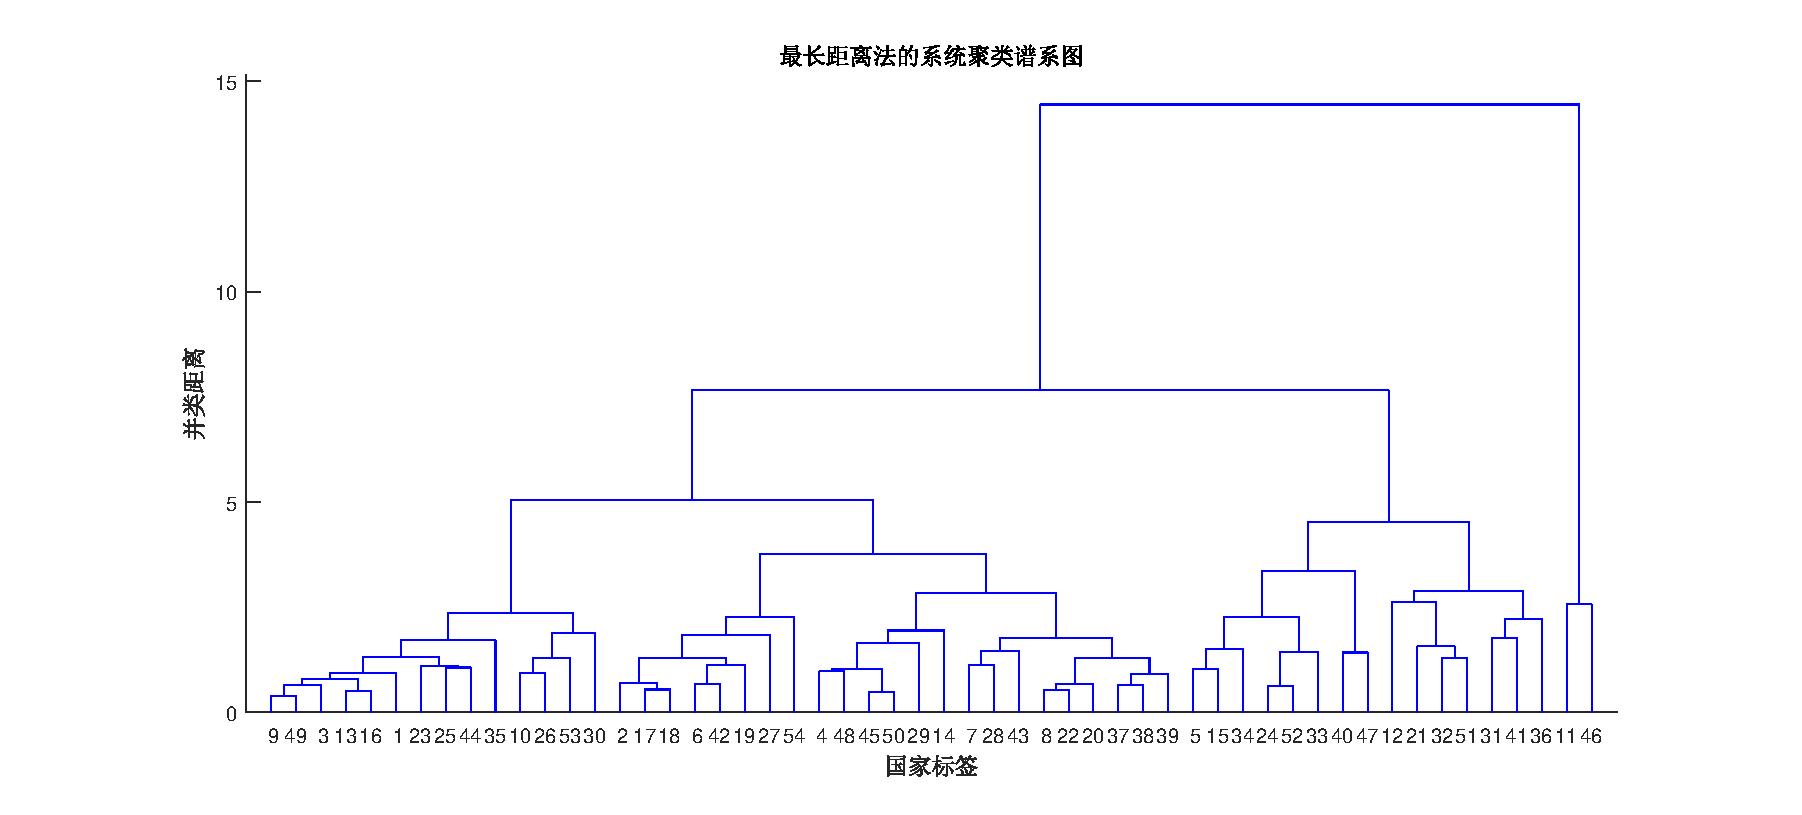
\includegraphics[scale=0.5]{dendrogram.eps}
\end{figure}

可以看到库克群岛和萨摩亚分到一类,而它们在各种排名方式下都是倒数后两名的队伍。
通过比较可以发现,其它三类与K-means分类法得到的结果大体一致。
\end{CJK}
\end{document}